% Chapter Template

\chapter{Performance Analysis and Comparison} % Main chapter title

\label{Chapter3} % Change X to a consecutive number; for referencing this chapter elsewhere, use \ref{ChapterX}

\fancyhead[RO]{\thepage}
\fancyhead[RE]{\thepage}
\fancyhead[LE]{Chapter 3.~\emph{\Chaptername}}
\fancyhead[LO]{\emph{\ttitle}}

%----------------------------------------------------------------------------------------
%	SECTION 1
%----------------------------------------------------------------------------------------

\section{Computational time comparison}
same program was run on different platforms with same simulation parameters. These platforms were GPU, MATLAB (CPU), c++ (CPU) more details about these platforms can be found in Appendix \ref{AppendixB}
Time domain is set to 1024,\\
Spatial domain values are $2^{10} - 2^{24}$,\\
\index{Performance comparison results, GPU C++ Matlab}
\begin{figure}[htbp]
	\centering
		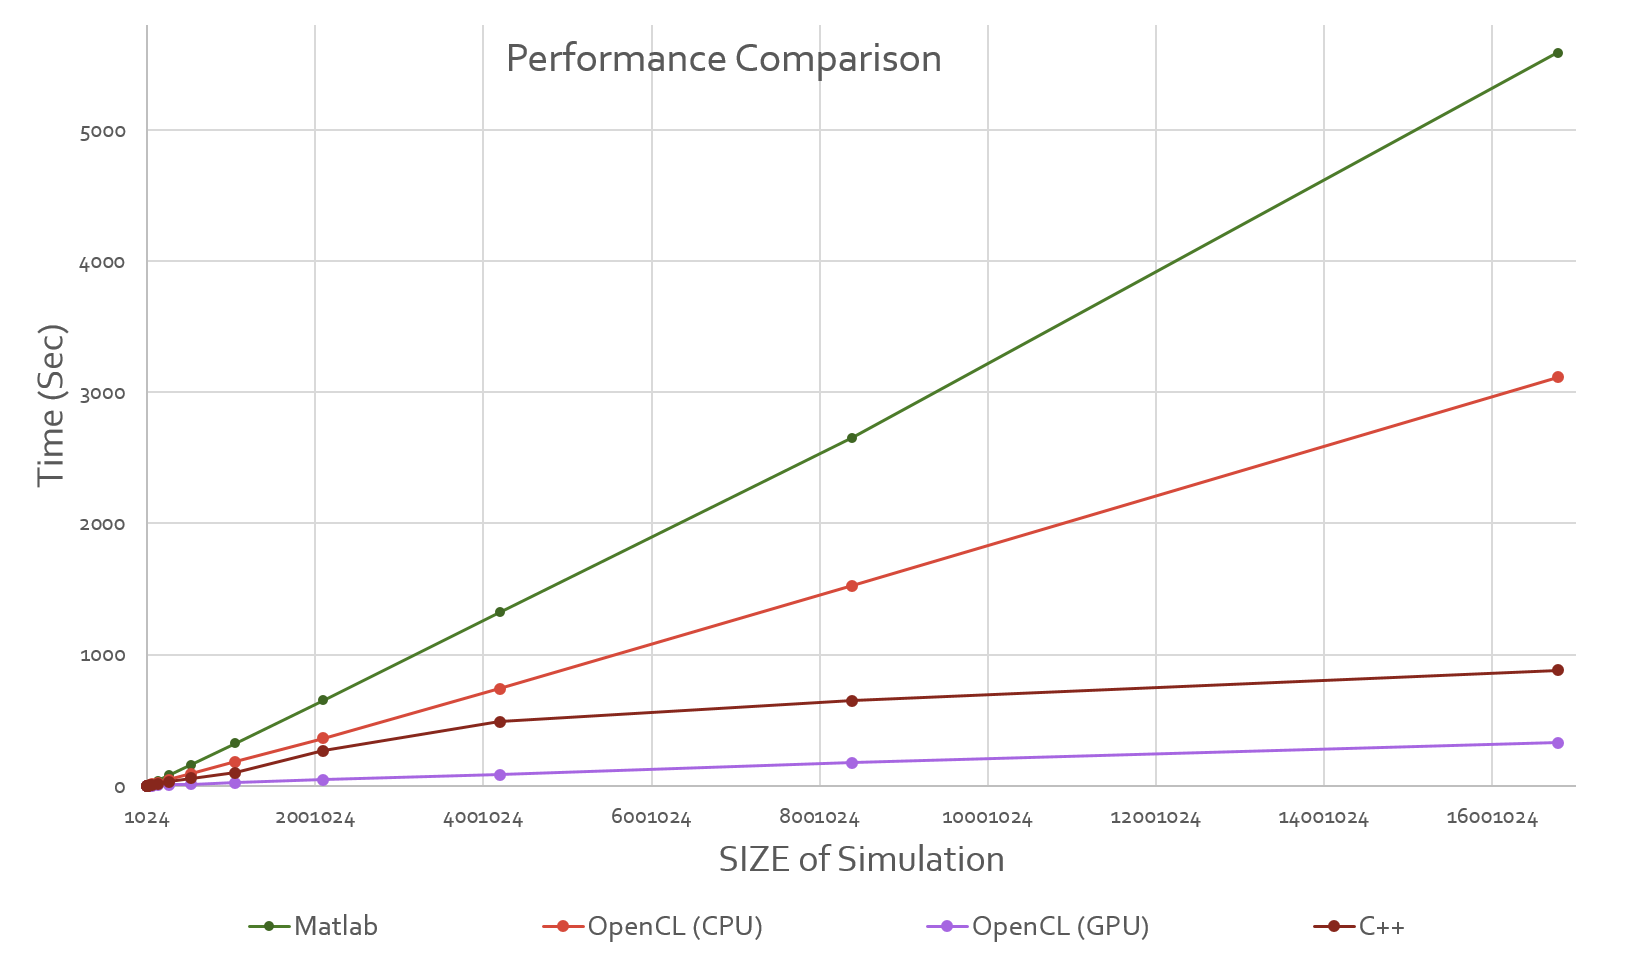
\includegraphics[width=6in]{Figures/g1.png}
	\caption[Computational Time on different platforms]{Performance comparison of computational time for different platforms over a large spatial domain $ Size = 2^{10} - 2^{24}$ }
	\label{g1}
\end{figure}
\begin{figure}[htbp]
	\centering
		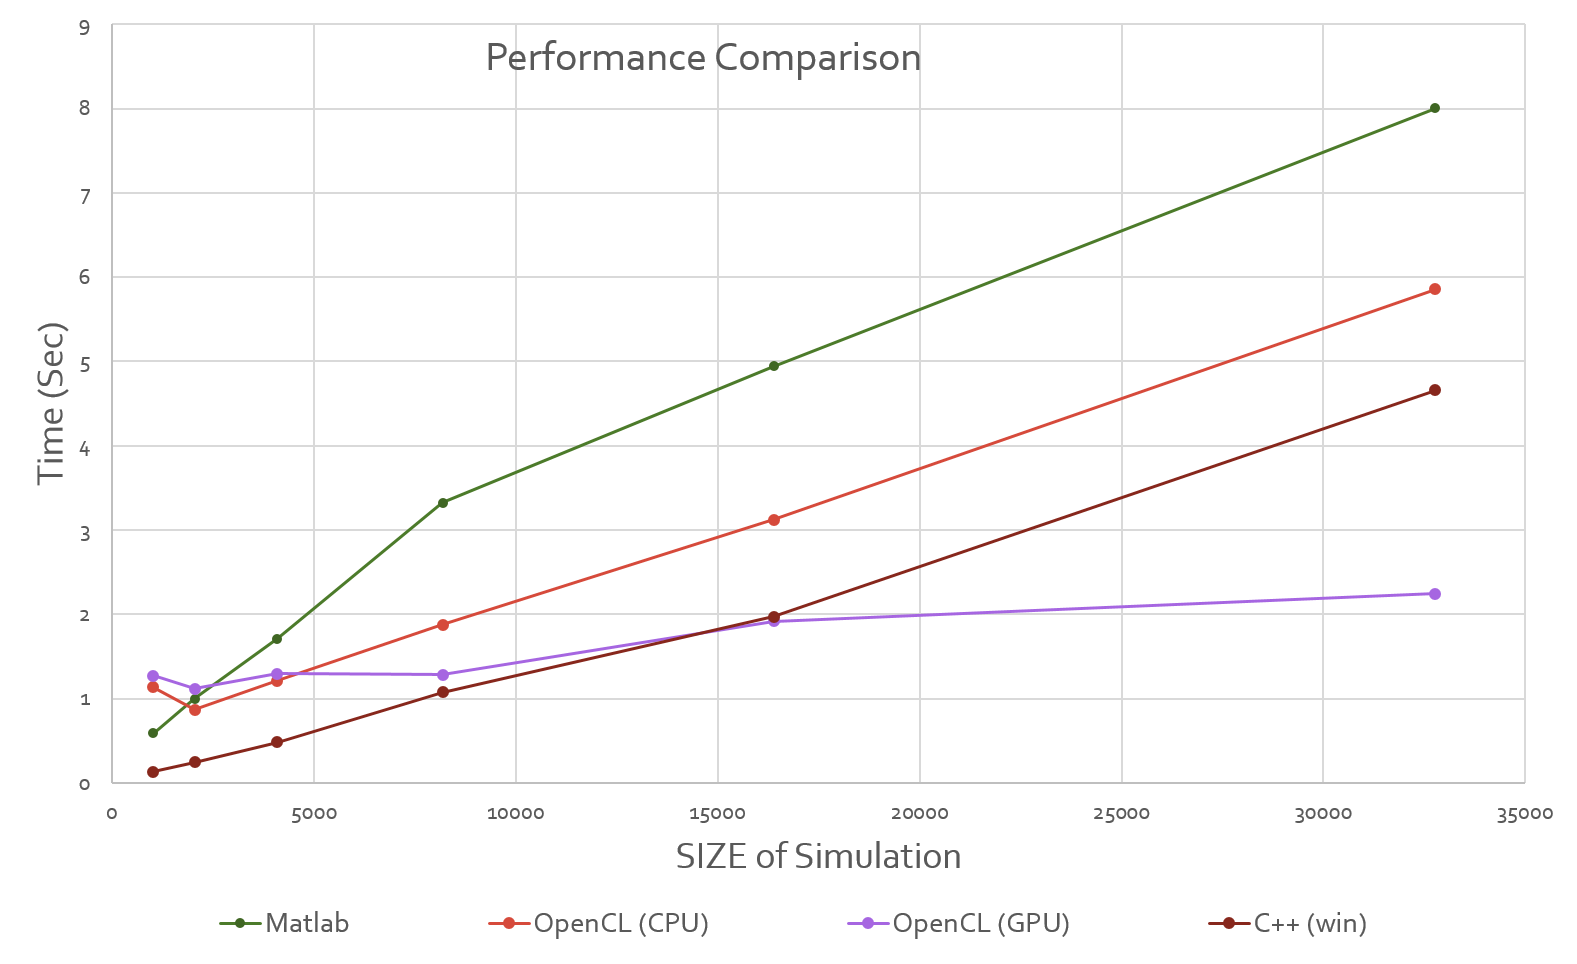
\includegraphics[width=6in]{Figures/g2.png}
	\caption[Computational Time on different platforms 2]{Performance comparison of computational time for different platforms for small size simulations $ Size = 2^{10} - 2^{15}$}
	\label{g2}
\end{figure}
\begin{figure}[htbp]
	\centering
		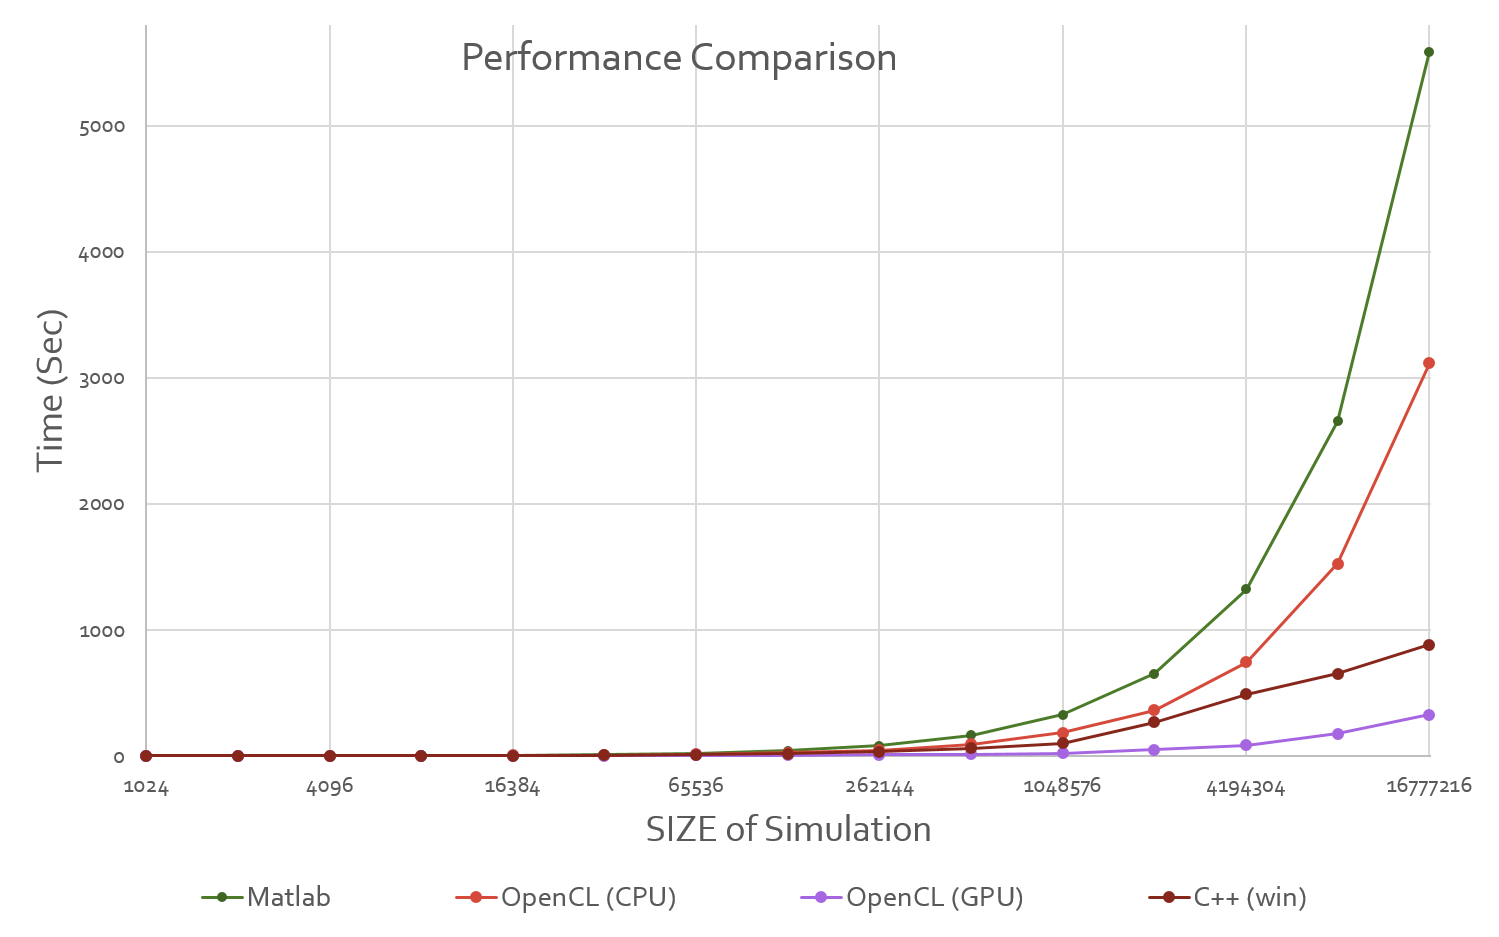
\includegraphics[width=6in]{Figures/g3.png}
	\caption[Performance Comparison on log scale]{Performance comparison of computational time for different platforms plotted over log scale}
	\label{g3}
\end{figure}

%-----------------------------------
%	SUBSECTION 2
%-----------------------------------
\section{Analysis }

From figure \ref{g1} it can be clearly observed that  computational time of GPU      is lowest and in term of few seconds even far larger domain size. it is 3 times better than that of C++ and           20 times better than MATLAB. These results can be improved by using a high end GPU or by using desktop version of GPU because in this case CPU (i7) is comparable to GPU (AMD 6770 Mobile).\\
Figure \ref{g2} shows the same results but it is plotted against on a relatively small domain size. here we can see the transitions in results. GPU is taking almost same time for lower simulation sizes this is because GPU takes some time to initialize  (see \nameref{HostProgram} on page \pageref{HostProgram}). the crossover point can be seen to be $2^{14}$.\\
Figure \ref{g3} shows the performance on a logarithmic $2^n$ x-axis, as we increase the domain size only in powers of two because of GPU kernels are in power of 2 and we do not want hardware resources to be underutilized. from this graph we can see the trend and also we can predict the computational time for each platform if we increase the domain size from $2^k  to  2^{k+1}$. 


%----------------------------------------------------------------------------------------
%	SECTION 2
%----------------------------------------------------------------------------------------

\section{Conclusion and Future Work}


%-----------------------------------
%	SUBSECTION 1
%-----------------------------------
\subsection{Conclusion }
FDTD algorithm was successfully implemented with Drudes model. All the parameters have been established and results are accurate when compared to theoretical values. Whole program was implemented on GPU and a significant reduction in computational time was achieved. it is observed that for small size simulations CPU gives a better performance than GPU, it also saves us from complex programming.


%-----------------------------------
%	SUBSECTION 2
%-----------------------------------
\subsection{Future Work }

There are number of applications of Negative index material, now that a basic platform is available and it is optimized for big simulations hence those applications can be modeled and researched further. Some interesting applications include Fiber optic design; for longer distances, RADAR absorbent; can be used in military applications as RAM, Photo-voltaic cell; with increased efficiency, Super lens; a lens with theoretical infinite zoom capabilities which can go beyond diffraction limits of conventional lens. the options are endless and with advancement of technology it is possible to not only research these fields but actually implement these modeled designs into physical designs. Negative index materials are a hot research topic in field of Electromagnetic field with a lot of known uses till date, it can be further explored for new uses and applications.

